Για την εκτίμηση της εξέλιξης της επίδοσης σε διάρκεια αγώνα, εκτελέστηκε προσομοίωση αγώνα $80$ διαδοχικών γύρων. Ο αριθμός των γύρων είναι μεγαλύτερος από την τυπική αναμενόμενη διάρκεια ζωής των ελαστικών, αλλά επιλέχθηκε με σκοπό τον εντοπισμό του σημείου όπου τα ελαστικά φτάνουν τη μέγιστη επιτρεπόμενη φθορά. Σε κάθε γύρο $k$ το διάγραμμα επιδόσεων ανανεώνεται με τη συνολική φθορά και τις αρχικές θερμοκρασίες των ελαστικών, που ταυτίζονται με τις τελικές του προηγούμενου γύρου. Έτσι αναπαράγεται ποιοτικά η τυπική τάση αύξησης του χρόνου γύρου με τη φθορά των ελαστικών, καθώς και η σταθεροποίηση των θερμοκρασιών λειτουργίας μετά τους πρώτους γύρους.\\[8pt]

\noindent
Στο \cref{fig:stintLapTimeVsLap} παρατηρείται η αναμενόμενη αύξηση του χρόνου γύρου κατά τη διάρκεια του αγώνα. Η αρχική μείωση του χρόνου στους πρώτους γύρους δεν οφείλεται στην άνοδο της θερμοκρασίας, αλλά στο φαινόμενο \textit{scrubbing-in} (\cref{subsubsec:wear_grip_coupling}), καθώς στην αρχική φάση φθοράς η πρόσφυση του ελαστικού αυξάνεται ελαφρά. Η απότομη αύξηση της κλίσης μετά τον γύρο $50$ αντιστοιχεί στο σημείο όπου ο συντελεστής μείωσης πρόσφυσης λόγω φθοράς εισέρχεται στην περιοχή απότομης πτώσης (\cref{fig:wear-scaling}). Η συνολική φθορά (\cref{fig:wearVsLap}) αυξάνεται σχεδόν γραμμικά με τον αριθμό των γύρων, ενώ η θερμοκρασία (\cref{fig:temperatureVsLap}) σταθεροποιείται σχεδόν αμέσως και παραμένει πρακτικά σταθερή καθ' όλη τη διάρκεια του αγώνα, με μεταβολή μικρότερη των $2\,^\circ\mathrm{C}$. Αυτό πιθανότατα οφείλεται, όπως και στη σύγκριση ψυχρού και θερμού γύρου, στη μοντελοποίηση μόνο της θερμικής μάζας του πέλματος, η οποία έχει ως αποτέλεσμα πολύ μικρή χρονική σταθερά.\\[8pt]
Τα ελαστικά φτάνουν τη μέγιστη επιτρεπόμενη φθορά αρκετά αργά, μετά από περίπου $55$ γύρους, γεγονός που είναι ασυνήθιστο δεδομένου ότι οι παράμετροι του μοντέλου βασίζονται σε μαλακή γόμα \cite{Tremlett2016}. Καθώς το μοντέλο φθοράς δεν έχει βαθμονομηθεί, και δεν υπάρχουν διαθέσιμα δεδομένα για αυτόν τον σκοπό, η απόκλιση μπορεί να οφείλεται σε αυτό, ή εναλλακτικά τα ελαστικά να είναι πράγματι ανθεκτικά στη φθορά. Αντίστοιχα, η απώλεια χρόνου γύρου δεν είναι ιδιαίτερα έντονη -- περίπου $0.3\,\mathrm{s}$ έως τη μέγιστη επιτρεπόμενη φθορά και περίπου $1\,\mathrm{s}$ στον γύρο $80$. Αυτό μπορεί να οφείλεται είτε στη μικρή ευαισθησία της πρόσφυσης των ελαστικών στη φθορά, είτε στο γεγονός ότι η πίστα \textit{Circuit de Barcelona-Catalunya} δεν εξαρτάται έντονα από την πρόσφυση: λόγω των πολλών μεγάλων ευθειών αποτελεί κυρίως πίστα ισχύος, όπου ο χρόνος γύρου καθορίζεται σε μεγάλο βαθμό από το όριο του κινητήρα και όχι από το διάγραμμα επιδόσεων.


\begin{figure}[htbp!]
    \centering
    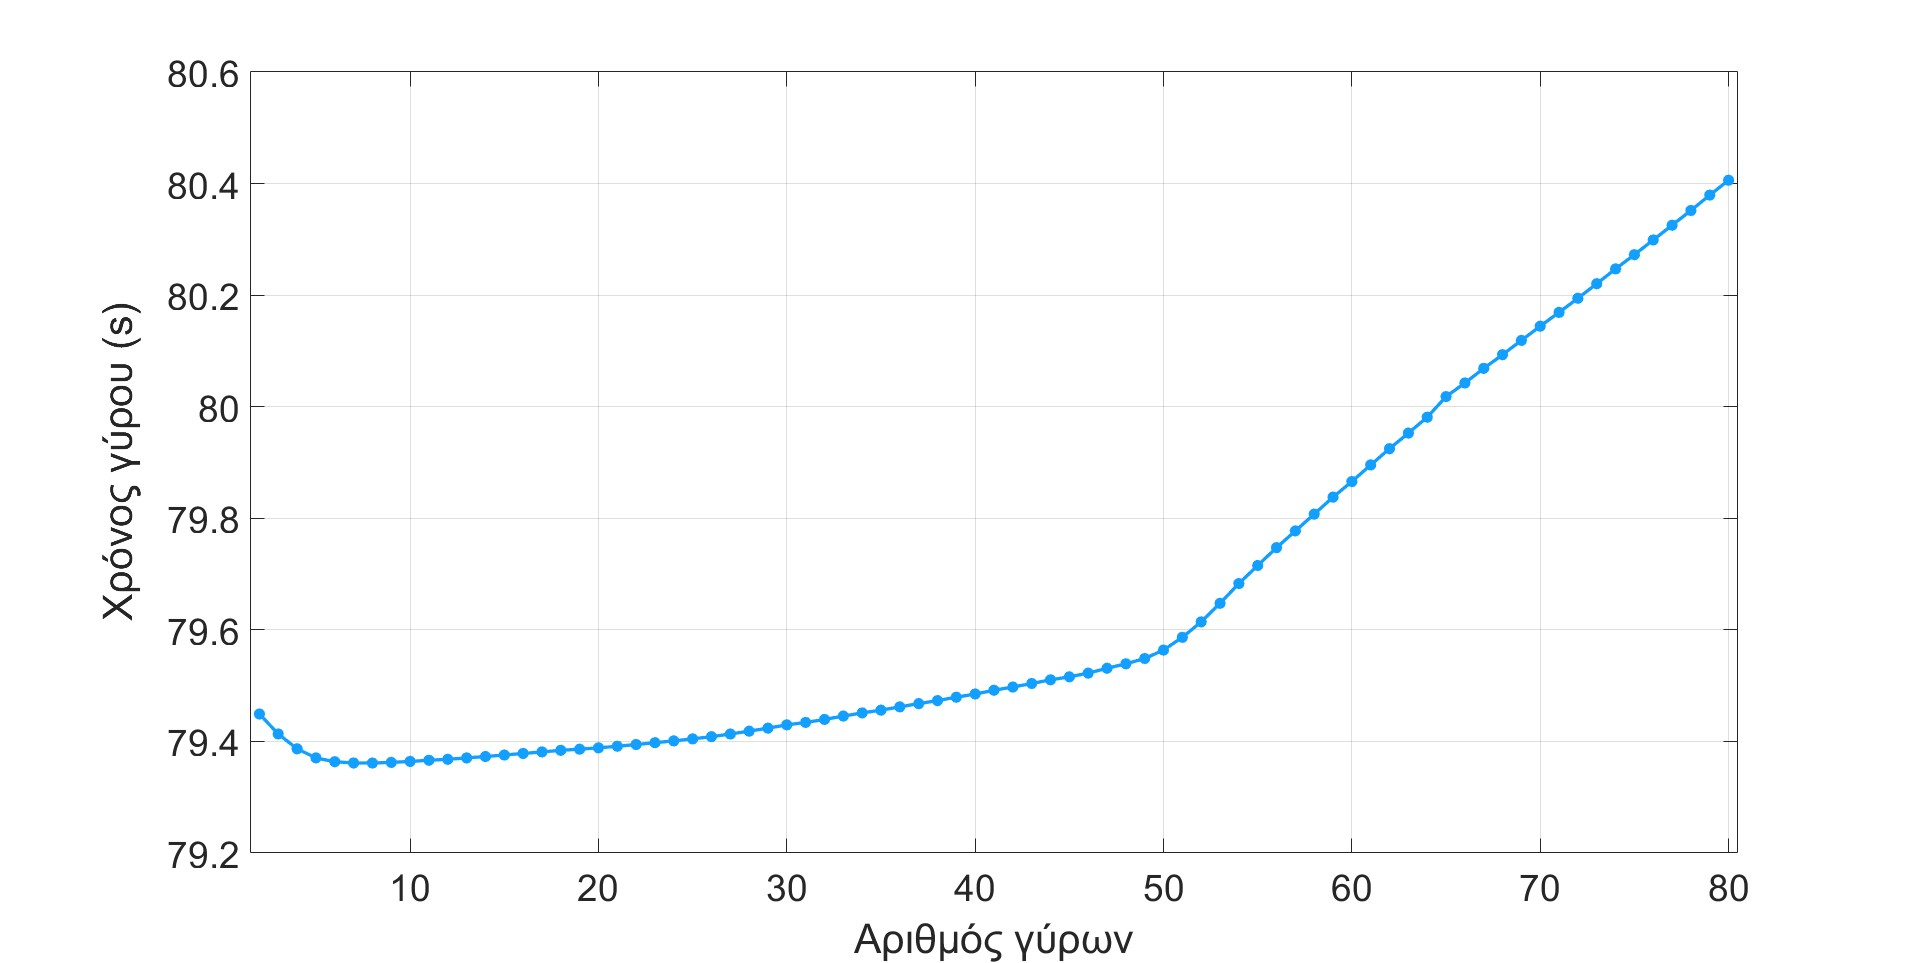
\includegraphics[width=0.7\textwidth]{figures/stint30laps/laptime_vs_lap.jpg}
    \caption{Χρόνος γύρου συναρτήσει του αριθμού των γύρων (\textit{Circuit
de Barcelona-Catalunya})}
    \label{fig:stintLapTimeVsLap}
\end{figure}

\begin{figure}[htbp!]
    \centering
    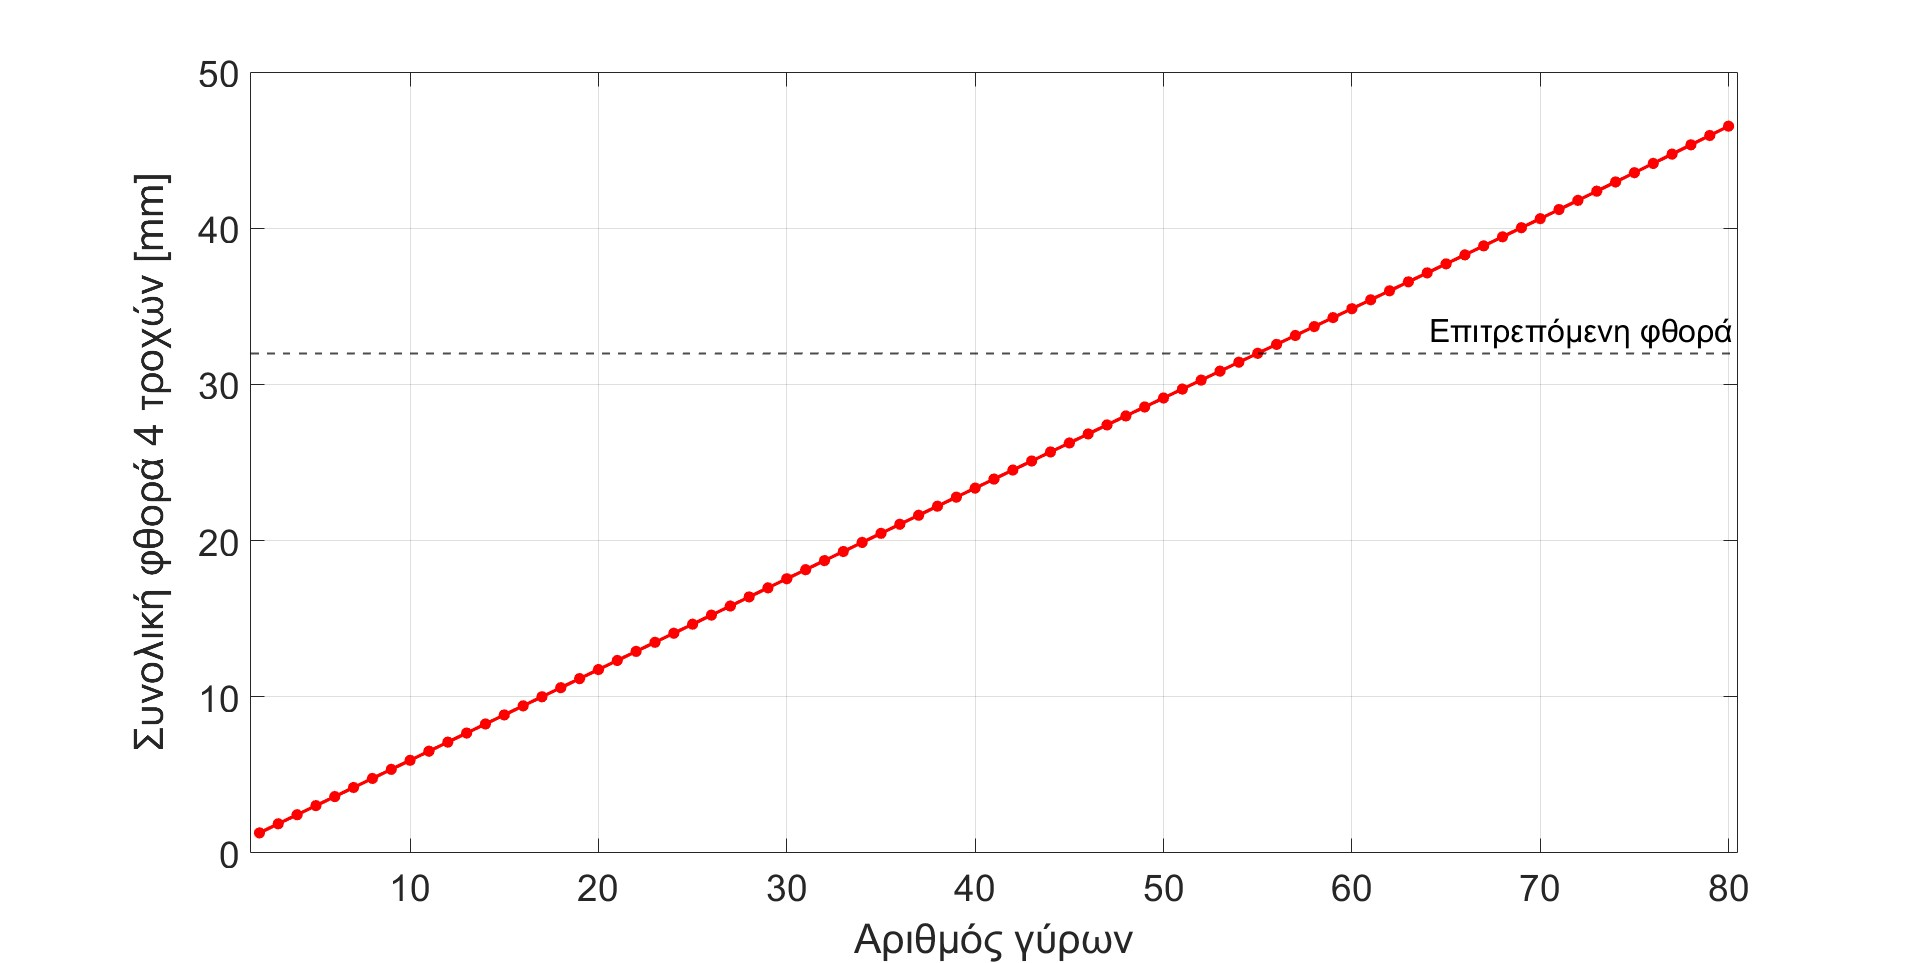
\includegraphics[width=0.7\textwidth]{figures/stint30laps/cumWear_vs_laptime.jpg}
    \caption{Συνολική φθορά συναρτήσει του αριθμού των γύρων (\textit{Circuit
de Barcelona-Catalunya})}
    \label{fig:wearVsLap}
\end{figure}

\begin{figure}[htbp!]
    \centering
    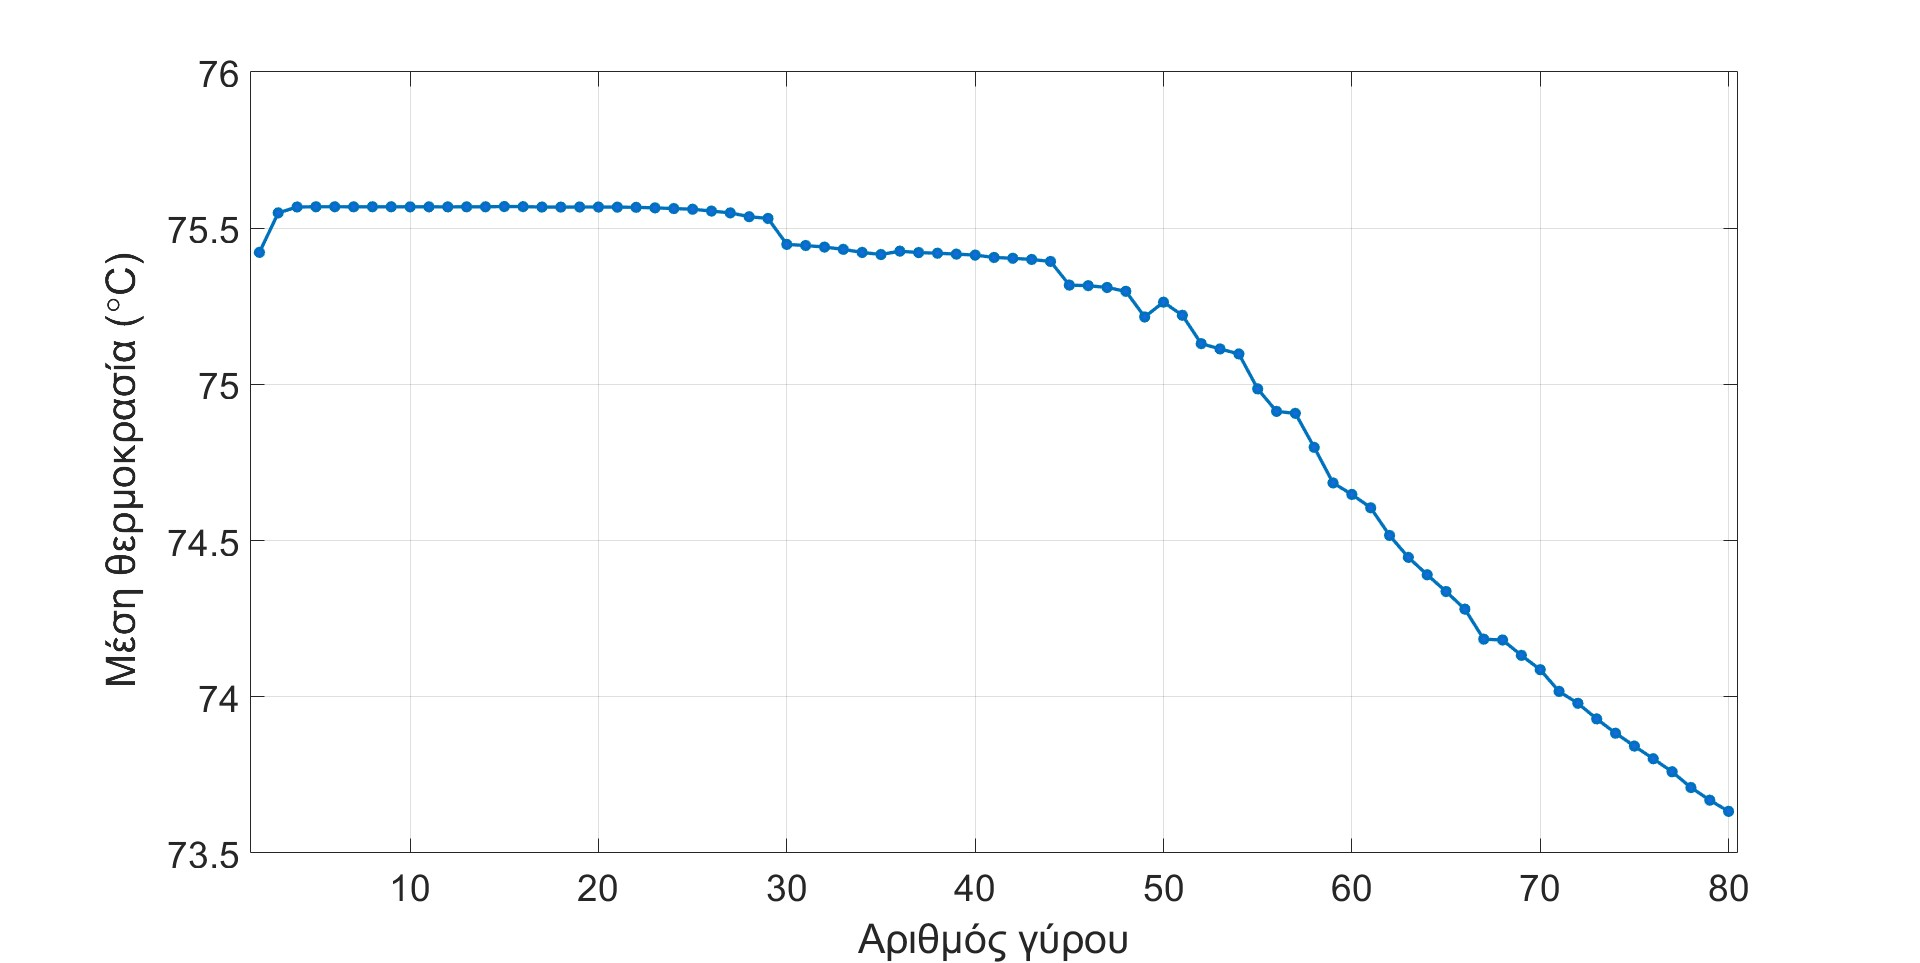
\includegraphics[width=0.7\textwidth]{figures/stint30laps/T_end_vs_lap.jpg}
    \caption{Μέση θερμοκρασία ελαστικών συναρτήσει του αριθμού των γύρων (\textit{Circuit
de Barcelona-Catalunya})}
    \label{fig:temperatureVsLap}
\end{figure}

\FloatBarrier
